\documentclass[12pt]{article}
\usepackage[utf8]{inputenc}
\usepackage{graphicx,setspace,csquotes}
\usepackage{float}
\usepackage[T1]{fontenc}
\usepackage[skip=12pt, indent=30pt]{parskip}
\usepackage[english]{babel}
\usepackage[autolanguage]{numprint}
\usepackage[backend=biber,style=apa,sorting=nyt]{biblatex}
\usepackage[font=small,labelfont=bf]{caption}
\usepackage[margin=2.5cm]{geometry}
\usepackage{booktabs}
\usepackage[english]{algorithm2e}
\usepackage{float}
\usepackage{hyperref}
\def\frenchtablename{Tableau}
\usepackage{caption}
\usepackage{subcaption}
\usepackage[dvipsnames]{xcolor}
\usepackage{listings}
\usepackage{listingsutf8}
\usepackage{ragged2e}
\usepackage{amsmath}
\usepackage{tocloft}
\usepackage{minted} 
%\usepackage{enumitem}

\addbibresource{biblio.bib}

\definecolor{grey}{RGB}{220, 220, 240}
\definecolor{personalizedColor}{RGB}{0, 163, 166}
\definecolor{codegreen}{rgb}{0,0.6,0}
\definecolor{codegray}{rgb}{0.5,0.5,0.5}
\definecolor{codepurple}{rgb}{0.58,0,0.82}
\definecolor{backcolour}{rgb}{0.95,0.95,0.92}

\lstdefinestyle{mystyle}{
    backgroundcolor=\color{backcolour},   
    commentstyle=\color{codegreen},
    keywordstyle=\color{magenta},
    numberstyle=\tiny\color{codegray},
    stringstyle=\color{codepurple},
    basicstyle=\ttfamily\footnotesize,
    breakatwhitespace=false,         
    breaklines=true,                 
    captionpos=b,                    
    keepspaces=true,                 
    numbers=left,                    
    numbersep=5pt,                  
    showspaces=false,                
    showstringspaces=false,
    showtabs=false,                  
    tabsize=2
}

\lstdefinestyle{DOS}
{
  basicstyle=\small\color{black},
  % numbers=left,
  % numberstyle=\tiny,
  % frame=tb,
  columns=fullflexible,
  breaklines=true,
  backgroundcolor=\color{grey},
}

    % backgroundcolor=\color{black},
    % basicstyle=\scriptsize\color{white}\ttfamily

% Configuration des liens
\hypersetup{
    colorlinks=true,
    linkcolor=black,
    filecolor=black,      
    urlcolor=personalizedColor,
    citecolor=personalizedColor,
    pdftitle={Titre du PDF},
    pdfpagemode=FullScreen,
    }
\urlstyle{same}
% Configuration des algorithmes
\RestyleAlgo{ruled}
\SetKw{KwBy}{by}
% Configuration des légendes
\captionsetup{width=13.5cm}

\begin{document}




\begin{titlepage}
    \begin{center}
        \vspace*{1cm}
        
        \Huge
        \textbf{Projet IA 2024/2025}
        
        \vspace{1.5cm}
        
        \LARGE
        \textbf{Safeband}
        
        \vspace{0.5cm}
        
        \Large
        Compte rendu d'avancement
        
        \vspace{0.5cm}
        
        \large
        Décembre 2024
        
        \vspace{1.5cm}
        
        
\includegraphics[width=0.7\textwidth]{logos/centraleSupelec.png}
        
        \vfill
        
        \hrule
        
        \vspace{0.5cm}
        
        \large
        \begin{tabbing}
            \hspace{7cm} \= \hspace{8cm} \kill
            Maceo Duriez \> \href{mailto:maceo.duriez@student-cs.fr}{maceo.duriez@student-cs.fr} \\
            Gaétan Jacquemin \> \href{mailto:gaetan.jacquemin@student-cs.fr}{gaetan.jacquemin@student-cs.fr} \\
            Ilann Amiaud-Plachy \> \href{mailto:ilann.amiaudplachy@student-cs.fr}{ilann.amiaudplachy@student-cs.fr}
        \end{tabbing}
        
        \vspace{0.5cm}
        
        \hrule
        
    \end{center}
\end{titlepage}




\tableofcontents{}

\newpage

\section{Étape 1 : Modélisation du Problème d'Assignation}

Le travail se fera pour 4 SR et 22 territoires à attribuer pour nous verrons si notre modèle tient à l'échelle pour 10 SR et 100 zones dans l'étape 2.

\subsection{Formulation des modèles mono-objectifs}
Dans un premier temps, deux modèles mathématiques sont formulés pour résoudre le problème d'assignation des représentants de vente aux territoires. 
Le premier modèle vise à minimiser la distance totale parcourue par les représentants, tandis que le second cherche à minimiser la perturbation causée par une nouvelle répartition des zones.

Soit :
\begin{itemize}
    \item $x_{ij}$ une variable binaire indiquant si la zone $i$ est assignée au représentant $j$.
    \item $d_{ij}$ la distance entre le centre du territoire du représentant $j$ et la zone $i$.
    \item $p_i$ la charge de travail nouvelle associée au changement de l'affectation de la zone $i$.
\end{itemize}

L'objectif de minimisation de la distance est donné par :
\begin{equation}
    \min \sum_{i,j} d_{ij} x_{ij}
\end{equation}
Cet objectif permet de minimiser la distance parcourue par l'ensemble des représentants, sans prendre en compte si la distance parcourue est équilibrée.

L'objectif de minimisation de la perturbation est donné par :
\begin{equation}
    \min \sum_{i} p_i x_{ij}
\end{equation}

Nous avons de même essayé un second objectif de minimisation pour la distance :
\begin{equation}
    \min \max \sum_{i,j} d_{ij} x_{ij}
\end{equation}
Cet objectif permet de rendre la répartition plus équitable, car on minimise la distance parcourue par le représentant qui en parcourt le maximum. Chaque représentant aura alors un travail plus équitable.

Sous contraintes :
\begin{itemize}
    \item Chaque zone est assignée à exactement un représentant.
    \item La charge de travail de chaque représentant est équilibrée (c'est à dire, inférieure à 1.2 et supérieure à 0.8).
    \item Les représentants ne peuvent pas être déplacés
\end{itemize}

\subsection{Résolution avec GUROBI}
Les modèles formulés sont implémentés et résolus avec l'optimiseur GUROBI. L'instance test comprend 22 zones et 4 représentants de vente.

Les étapes de l'implémentation incluent :
\begin{itemize}
    \item Définition des variables de décision.
    \item Définition des contraintes du modèle.
    \item Résolution et analyse des solutions obtenues.
\end{itemize}

La solution pour la minimisation mono-objective de la nouvelle charge de travail (disruption) donne une valeur de 0.170.

La solution optimale du mono-objectif de minimisation de la distance totale donne une valeur de 56. 

Pour pouvoir transformer l'optimisation non linéaire du Min(Max), il suffit seulement de rajouter une variable $z$ qui est le maximum de toutes les distances parcourues par les représentants. On peut alors ajouter une contrainte pour que $z$ soit supérieur à toutes les distances parcourues par les représentants.
\subsection{Exploration des solutions non-dominées}
Une approche par contrainte-épsilon est utilisée pour générer l’ensemble des solutions non-dominées. L’idée est d’imposer des contraintes successives sur l’un des objectifs (la distance totale)  tout en minimisant l’autre (disruption).

L’analyse est réalisée avec trois niveaux de contraintes sur la charge de travail :
\begin{itemize}
    \item 1. [0.8, 1.2]
    \item 2. [0.85, 1.15]
    \item 3. [0.9, 1.1]
\end{itemize}

Chaque ensemble de solutions est visualisé à l’aide de graphes comparant la distance et la perturbation ci-dessous :

\begin{figure}[H]
    \centering
    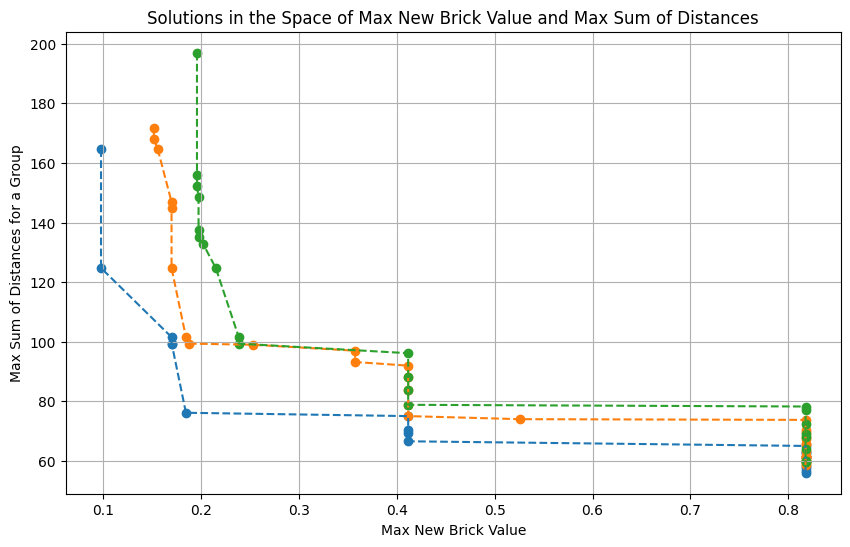
\includegraphics[width=\textwidth]{Images/step_1/step_1-min-distance.png}
    \caption{Solutions non-dominées avec l'objectif de distance Min pour des charges de travail selon 1. en bleu, 2. en orange et 3. en vert}
    \label{fig:nom_de_reference}
\end{figure}

\begin{figure}[H]
    \centering
    \includegraphics[width=\textwidth]{Images/step_1/step_1-min-distance-2.png}
    \caption{Solutions non-dominées avec l'objectif de distance MinMax pour des charges de travail selon 1. en bleu, 2. en orange et 3. en vert}
    \label{fig:nom_de_reference}
\end{figure}

La première figure est produite en optimisant le workload en principal et la distance en epsilon, et la seconde l'inverse, ce qui donne des différences notables.
\newpage

\section{Étape 3 : Optimisation de la Localisation des Bureaux}
\subsection{Modélisation bi-objective}
Dans cette étape, la localisation des bureaux des représentants de vente est prise en compte comme une variable de décision supplémentaire.
L'objectif est de minimiser simultanément la distance totale parcourue et de répartir équitablement la charge de travail entre les représentants.

Soit :
\begin{itemize}
    \item $y_j$ la position du bureau du représentant $j$.
    \item $c_{jk}$ la distance entre le nouveau bureau $y_j$ et la zone $k$.
\end{itemize}

On a donc de nouveau un critère bi-objectif mais cette fois avec plus de données en entrée. 
Le premier objectif est la minimisation de la distance totale parcourue par les SR et le second objectif est la minimisation de la charge de travail maximale d'un SR. En résolvant avec Gurobi, on trouve cet espace de solutions :
\begin{figure}[H]
    \centering
    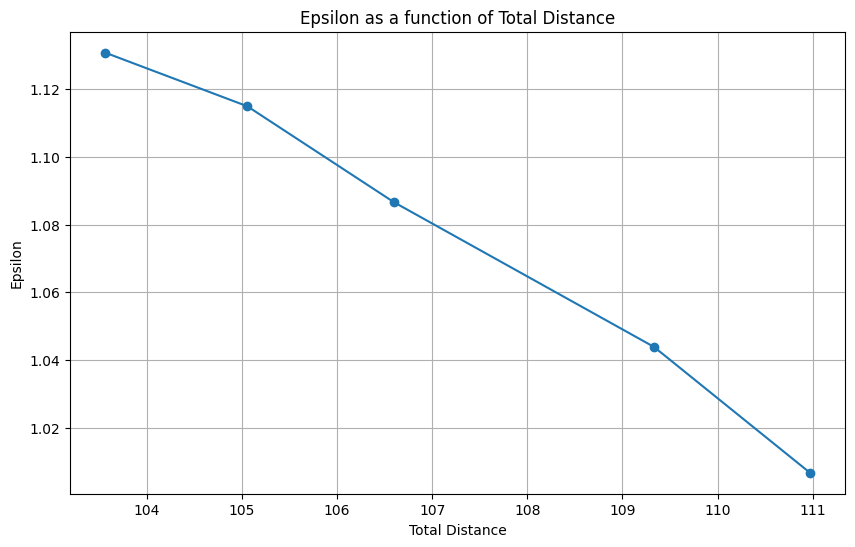
\includegraphics[width=\textwidth]{Images/step_3/bi-objective-moivng-office.png}
    \caption{Solutions non-dominées du problème bi-objectif avec la distance totale en abscisses et le MinMax de charge de travail en ordonnées}
    \label{fig:nom_de_reference}
\end{figure}


\subsection{Nouvelle disruption, nouveaux objectifs}

Maintenant, la disruption est redéfinie en termes de nombre d'office déplacé. Ainsi, le problème initial de cette étape devient tri-objectif. Comme la disruption ne peut prendre que des valeurs entières allant de 0 à 4, nous représentons les solutions non-dominées comme les graphes de solutions non-dominées bi-objectives (distance et charge de travail), à nombre d'offices changés déterminée. Voici alors l'espace des solutions :

\begin{figure}[H]
    \centering
    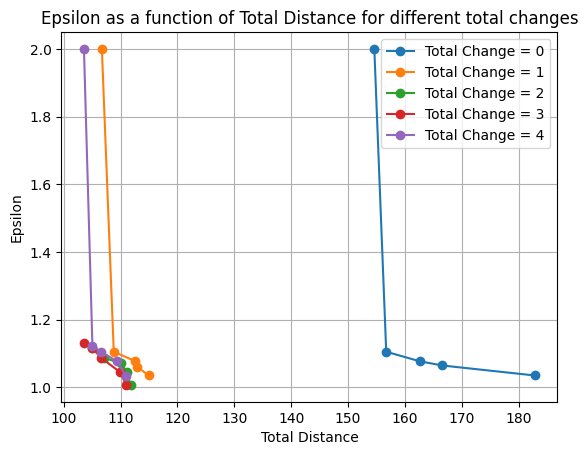
\includegraphics[width=\textwidth]{Images/step_3/tri-objectif.png}
    \caption{Solutions non-dominées du problème tri-objectif où epsilon représente le max de charge de travail pour un SR}
    \label{fig:nom_de_reference}
\end{figure}


\newpage



\end{document}


